\documentclass[a4paper,12pt]{article} % тип документа

% Поля страниц
\usepackage[left=2.5cm,right=2.5cm,
    top=2cm,bottom=2cm,bindingoffset=0cm]{geometry}
    
%Пакет дял таблиц   
\usepackage{multirow} 
    
%Отступ после заголовка    
\usepackage{indentfirst}


% Рисунки
\usepackage{floatrow,graphicx,calc}
\usepackage{wrapfig}

%%% Работа с картинками
\usepackage{graphicx}  % Для вставки рисунков
\graphicspath{{images/}}  % папки с картинками
\setlength\fboxsep{3pt} % Отступ рамки \fbox{} от рисунка
\setlength\fboxrule{1pt} % Толщина линий рамки \fbox{}
\usepackage{wrapfig} % Обтекание рисунков и таблиц текстом

% Создаём новый разделитель
\DeclareFloatSeparators{mysep}{\hspace{1cm}}

% Ссылки?
\usepackage{hyperref}
\usepackage[rgb]{xcolor}
\hypersetup{				% Гиперссылки
    colorlinks=true,       	% false: ссылки в рамках
	urlcolor=blue          % на URL
}


%  Русский язык
\usepackage[T2A]{fontenc}			% кодировка
\usepackage[utf8]{inputenc}			% кодировка исходного текста
\usepackage[english,russian]{babel}	% локализация и переносы

% Математика
\usepackage{amsmath,amsfonts,amssymb,amsthm,mathtools}

%%% Дополнительная работа с математикой
\usepackage{amsmath,amsfonts,amssymb,amsthm,mathtools} % AMS
\usepackage{icomma} % "Умная" запятая: $0,2$ --- число, $0, 2$ --- перечисление

% Что-то 
\usepackage{wasysym}


\begin{document}
\begin{center}
	\footnotesize{ФЕДЕРАЛЬНОЕ ГОСУДАРСТВЕННОЕ АВТОНОМНОЕ ОБРАЗОВАТЕЛЬНОЕ 			УЧРЕЖДЕНИЕ ВЫСШЕГО ОБРАЗОВАНИЯ}\\
	\footnotesize{МОСКОВСКИЙ ФИЗИКО-ТЕХНИЧЕСКИЙ ИНСТИТУТ\\(НАЦИОНАЛЬНЫЙ 			ИССЛЕДОВАТЕЛЬСКИЙ УНИВЕРСИТЕТ)}\\
	\footnotesize{ФИЗТЕХ-ШКОЛА ФИЗИКИ И ИССЛЕДОВАНИЙ им. ЛАНДАУ\\}
	\hfill \break
	\hfill \break
	\hfill \break
	\hfill \break
\end{center}

\begin{center}   
    \hfill \break
	\hfill \break
	\hfill \break
	\hfill \break    \hfill \break
	\hfill \break
	\hfill \break
	\hfill \break
    \hfill \break
    \hfill \break
	\hfill \break
	\large{Лабораторная работа № 2.5.1 \\\textbf{Измерение коэффициента поверхностного натяжения
  жидкости}}\\
	\begin{flushright}
		Плотникова Анастасия Александровна\\
		Группа Б02-406
	\end{flushright}
	\hfill \break
	\hfill \break
	\hfill \break
\end{center}
\hfill \break
\hfill \break
\hfill \break
\hfill \break
\hfill \break
\hfill \break
\hfill \break
\hfill \break
\hfill \break
\hfill \break
\hfill \break
\hfill \break
\hfill \break
\begin{center}
	Долгопрудный, 2025 г.
\end{center}
\thispagestyle{empty}
\newpage
	\textbf{Цель работы:}\\ 
  1) измерение коэффициента поверхностного натяжения исследуемой жидкости при разной температуре с использованием известного коэффициента поверхностного натяжения другой жидкости; \\
  2) определение полной поверхностной энергии и теплоты, необходимой для изотермического образования единицы поверхности жидкости.
	\hfill \break
	
	\textbf{В работе используются:}\\ 
  прибор Ребиндера, оснащенный \\
  — микроманометром, \\
  — термостатом LOIP LT-100 (установления: $dT = 0.2 ^\circ C$, поддержания: $dT = 0.1 ^\circ C$); \\
  исследуемые жидкости (спирт этиловый, вода дистиллированная); \\
  стакан; \\
  микроскоп.
	
\section*{Теоретическая справка}

\subsection*{Формула Лапласа}

Наличие поверхностного слоя приводит к различию давлений по разные стороны от искривленной границы раздела двух сред. Для сферического пузырька с воздухом внутри жидкости избыточное давление даётся формулой Лапласа:

\[
  \Delta P = \frac{2\sigma}{r} 
\]
где $\sigma$ –- коэффициент поверхностного натяжения, \\
$\Delta P$ – разница давлений внутри и снаружи пузырька, \\
$r$ – радиус кривизны поверхности раздела двух фаз. 

\subsection*{Закон Кирхгофа}

\[
  L(T) = L(T_0) + \int_{T_0}^{T}(C_{p \text{(п)}} - C_{p \text{(ж)}}) dT 
\]
\[
  L(T) = L(T_0) + (C_{p \text{(п)}} - C_{p \text{(ж)}}) (T - T_0)
\]



\section*{Экспериментальная установка} 

Схема установки изображена на рисунке (\ref{fig:setup}). 

\begin{figure}[h!]
  \centering
  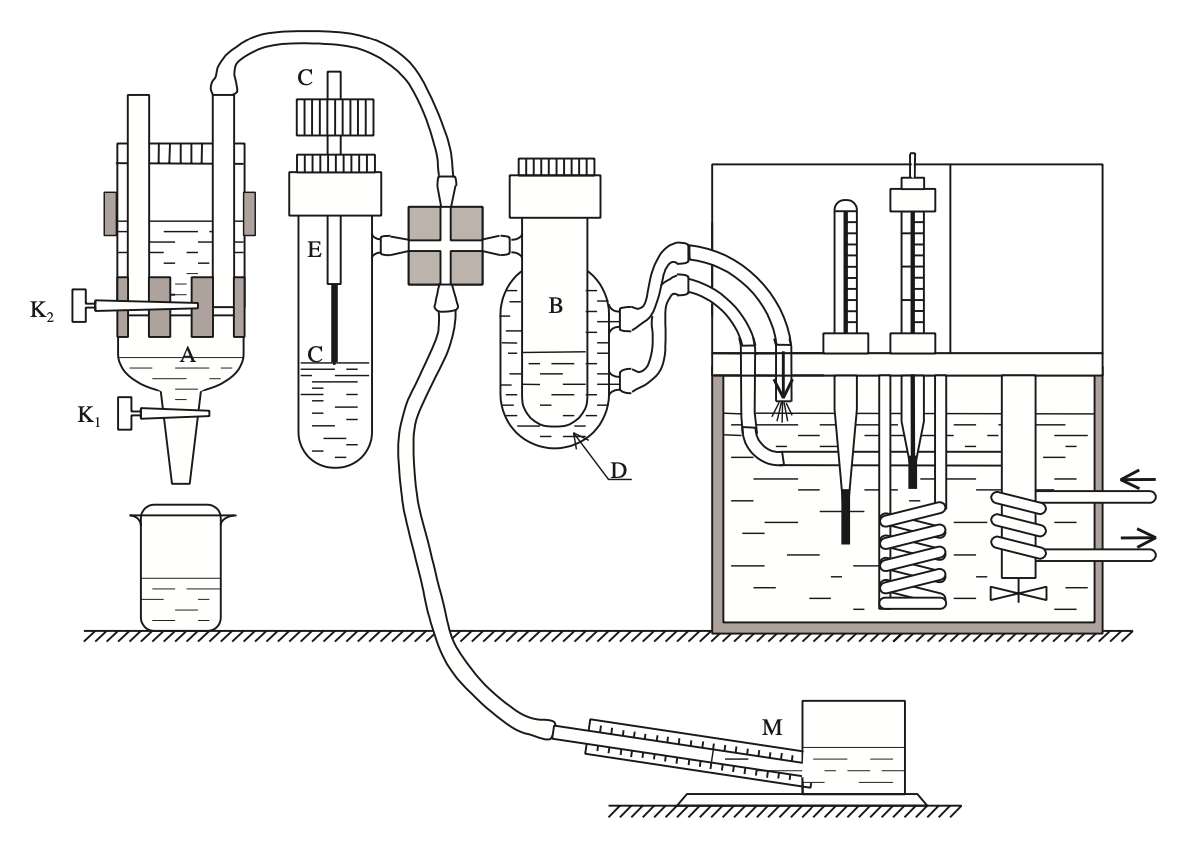
\includegraphics[scale = 0.75]{setup.png}
  \caption{Схема установки для измерения температурной зависимости коэффициента поверхностного натяжения.}
  \label{fig:setup}
\end{figure}

Исследуемая жидкость наливается в сосуд B, дистиллированная вода – в сосуд E. Через герметично закрытую пробку сосуда с иглой C создаётся разрежение, и воздух пробулькивает через жидкость. Поверхностное натяжение определяется по величине разрежения.

При приоткрытом кране K1 из аспиратора A вытекает вода, создавая разрежение, измеряемое манометром M. Его показания, умноженные на коэффициент (обычно 0,2), дают давление в $\text{кгс}/\text{м}^2$ ($1 \text{ кгс}/\text{м}^2 = 9{,}8 \text{ Па}$). Для пополнения воды кран K2 соединяет нижнюю часть аспиратора с атмосферой.

Температура стабилизируется водой из термостата через рубашку D. Игла обычно касается поверхности жидкости, но при измерении температурной зависимости натяжения возникают сложности: охлаждение конца иглы и тепловое расширение жидкости. Эти погрешности устраняются, если опустить иглу до дна.

Давление определяется как:
\[
P = \Delta P + \rho g h.
\]
Для измерения $\rho g h$ используются два метода:
\begin{enumerate}
    \item Определение $P_1$ при касании поверхности и $P_2$ при погружении до дна ($\rho g h = P_2 - P_1$).
    \item Измерение $h_1$ и $h_2$ при $P_1$ и $P_2$.
\end{enumerate}

Чувствительность микроманометров высока, поэтому перед изменениями в установке их переключают на атмосферу. При заполнении аспиратора без сброса давления возможны пузыри, нарушающие калибровку и точность измерений.



\section*{Ход работы}

\begin{enumerate}
  \item Убедимся в исправности установки. Аспиратор был заполнен водой, а чистая сухая игла установлена в сосуде со спиртом, не касаясь поверхности воды. Опустим иглу так, чтобы её кончик едва коснулся поверхности воды. Установим скорость падения капель примерно 1 капля в 3 секунды. Откроем кран аспиратора, заметим пробулькивания пузырьков воздуха в колбе. Манометр показывает медленный рост давления до некоторого максимального значения и затем быстрое его падение при пробулькивании пузырька.
  
  \item Подберём частоту падения капель так, чтобы максимальное давление не зависело от этой частоты. Для этого пузырьки не должны пробулькивать слишком часто (примерно 1 пузырёк в 3-5 секунд).
  
  \item Измерим максимальное давление при пробулькивании пузырька. Для точности проведем десять измерений и усредним полученное значение. Результаты представлены в таблице (\ref{tab:alcohol}).
  
  \begin{table}[h!]
    \centering
    \begin{tabular}{|c|cccccccccc|c|c|}
      \hline
      $h_\text{сп}$, мм & 47 & 47 & 47 & 47 & 48 & 47 & 48 & 47 & 47 & 47 & 47.2 & $\sigma_h = 1$ \\
      \hline
    \end{tabular}
    \caption{}
    \label{tab:alcohol}
  \end{table}
  
  По разбросу результатов оценим случайную погрешность ($\varepsilon_{h_\text{сп}} = 0.032$).

  \[
    h_\text{сп} = (47 \pm 2) \, \text{мм} = (4.7 \pm 0.2) \cdot 10^{-2} \, \text{м}
  \]

  Комнатная температура: $t = (24.8 \pm 0.3)^{\circ} C = (298.0 \pm 0.3) K $ \\
  Коэффициент поверхностного натяжения спирта (для $t \approx 25^{\circ}C$): 
  \[
    \sigma_\text{сп} = \frac{1}{2} (22.87 + 21.90) = 22.39 \, \frac{\text{мН}}{\text{м}}
  \] 
  \[ 
    d(\sigma_\text{сп}) = \frac{1}{2} (22.87 - 21.90) + 0.02 = 0.49 + 0.02 = 0.51 \, \frac{\text{мН}}{\text{м}}
  \]
  \[
    \sigma_\text{сп} = (22.4 \pm 0.5) \, \frac{\text{мН}}{\text{м}} = (2.24 \pm 0.05) \cdot 10^{-4} \, \frac{\text{Н}}{\text{м}}
  \]
  
  Плотность спирта (для $t \approx 25^{\circ}C$):  
  \[
    \rho_\text{сп} = \frac{1}{2} (789.5 + 781.0) = 785.3 \, \frac{\text{кг}}{\text{м}^3}
  \] 
  \[ 
    d(\rho_\text{сп}) = \frac{1}{2} (789.5 - 781.0) + 0.2 = 4.3 + 0.2 = 4.5 \, \frac{\text{кг}}{\text{м}^3}
  \]
  \[
    \rho_\text{сп} = (785 \pm 5) \frac{\text{кг}}{\text{м}^3} = (7.85 \pm 0.05) \cdot 10^{-2} \, \frac{\text{кг}}{\text{м}^3}
  \]
  
  Пользуясь табличным значением коэффициента поверхностного натяжения воды, определим диаметр иглы.

  \[
    \Delta P = \frac{2 \sigma_\text{сп}}{r} = \frac{4 \sigma}{d}, \quad d = \frac{4 \sigma}{\Delta P} = \frac{4 \sigma}{\rho_\text{сп} g l \sin{\alpha}} = 1.238 \cdot 10^{-3} \, \text{м}
  \]
  \[ 
    \varepsilon_{d} = \sqrt{\varepsilon_{\sigma}^2 + \varepsilon_{\rho_\text{сп}}^2 + \varepsilon_{l}^2} = 0.031, \quad d(d) = d \cdot \varepsilon_{d} = 3.9 \cdot 10^{-5} \, \text{м}
  \]
  \[ 
    d = (1240 \pm 40) \, \text{мм} = (1.24 \pm 0.04) \cdot 10^{3} \, \text{м}
  \]

  Проверим применимость формулы Лапласа. Сравним полученный результат с прямыми измерениями диаметра иглы, представленными на рисунке (\ref{fig:needle}). Провели два измерения, значения совпали. К сожалению, только одно из измерений получилось качественно запечатлеть на фотографии.

  \begin{figure}[h]
    \centering
    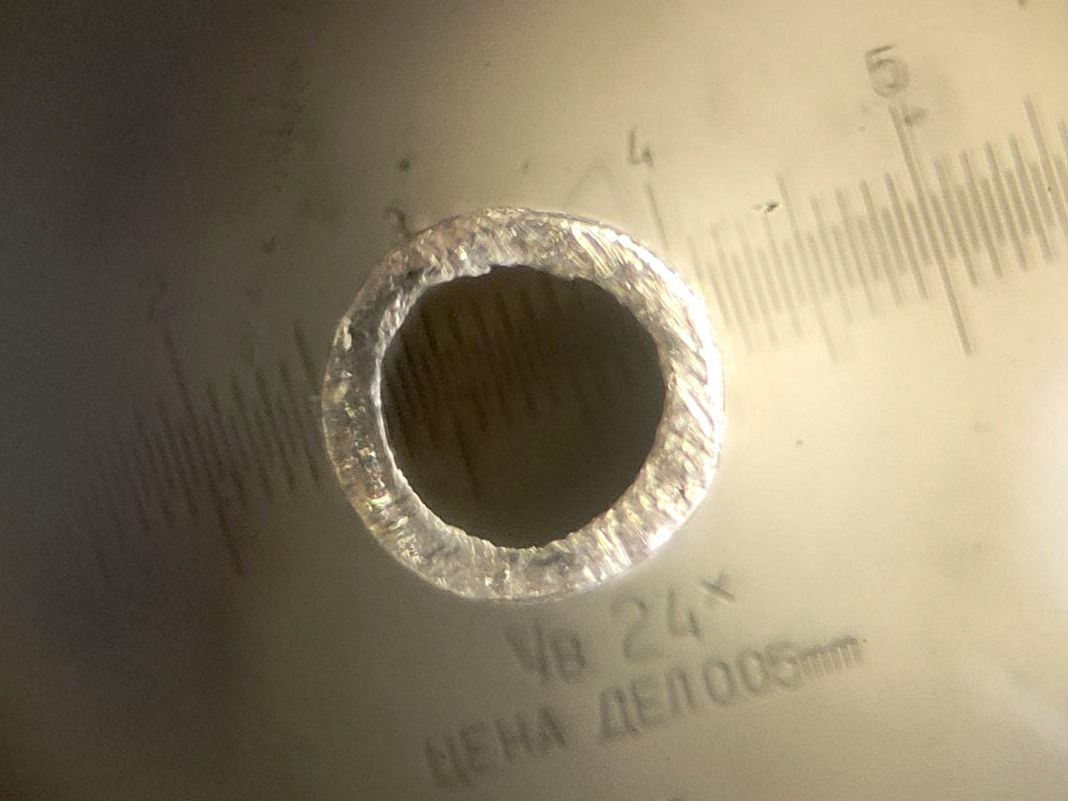
\includegraphics[scale = 0.2]{needle.jpg}
    \caption{Изображение разреза иглы в увеличении микроскопа}
    \label{fig:needle}
  \end{figure}

  \[
    d = (1.1 \pm 0.1) \, \text{мм} = (1.1 \pm 0.1) \cdot 10^{-3} \, \text{м}
  \]

  Значения совпадают в пределах погрешности. Формула Лапласа верна с достаточной точностью.
  
  \item Перенесём иглу в сосуд с дистиллированной водой. Измерим максимальное давление в пузырьках, когда игла лишь касается поверхности жидкости. Измерим $h_1 = h_\text{в}$ десять раз, занесем полученные значения в таблицу (\ref{tab:water1}). 
  
  \begin{table}[h!]
    \centering
    \begin{tabular}{|c|cccccccccc|c|c|}
      \hline
      $h_1$, мм & 125 & 124 & 125 & 125 & 125 & 125 & 125 & 125 & 125 & 125 & 125.1 & $\sigma_h = 1$ \\
      \hline
    \end{tabular}
    \caption{}
    \label{tab:water1}
  \end{table}

  Рассчитаем случайную погрешность ($\varepsilon_{h_1} = 0.018$).

  \[
    h_1 = (125 \pm 2) \, \text{мм} = (1.25 \pm 0.02) \cdot 10^{-1} \, \text{мм}
  \]
  \[
    \Delta P_1 = \rho_\text{сп} g h_1 \sin{\alpha} = 192.52 \, \text{Па} 
  \]
  \[
    \Delta P_1 = (193 \pm 5) \, \text{Па} = (1.93 \pm 0.05) \cdot 10^{2} \, \text{Па} \qquad (2.4 \%)
  \]

  Сравним с результатом, выраженным через табличные величины.

  \[
    d \sim \frac{\sigma}{h} \Longrightarrow \frac{\sigma_\text{сп}}{h_\text{сп}} = \frac{\sigma_\text{в}}{h_\text{в}} 
  \]
  \[
     h_\text{в} = h_\text{сп} \frac{\sigma_\text{в}}{\sigma_\text{сп}} = 47 \cdot 10^{-3} \frac{(72.0 \pm 0.5) \cdot 10^{-3}}{(22.4 \pm 0.5) \cdot 10^{-3}} = (151 \pm 3) \, \text{мм} = (1.51 \pm 0.03) \cdot 10^{-1} \, \text{м}
  \]

  Значения различаются на $20 \%$, порядок совпадает. 

  \item Утопим иглу до предела, насколько это позволяет установка. Между концом иглы и дном останется небольшой зазор, так, образующийся пузырёк не будет касаться дна.

  Измерим расстояние от верхней части установки до подвижной части крепления иглы до и после установки по два раза (совпали, случайную погрешность не учитываем). Его изменение равно глубине погружения.
  \[
    h_1 = (17 \pm 1) \, \text{мм}, \quad h_2 = (6 \pm 1) \, \text{мм}
  \]
  \[
    \Delta h = h_1 - h_2 = (11 \pm 2) \, \text{мм}
  \]

  Измерим максимальное давление в пузырьках. По разности давлений в этом и предыдущем пункте определим глубину погружения. Измерим $h_2$. Полученные давления представлены в таблице (\ref{tab:water2}).

  \begin{table}[h!]
    \centering
    \begin{tabular}{|c|cccccccccc|c|c|}
      \hline
      $h_2$, мм & 196 & 196 & 197 & 196 & 196 & 196 & 196 & 196 & 196 & 195 & 196.0 & $\sigma_h = 1$ \\
      \hline
    \end{tabular}
    \caption{}
    \label{tab:water2}
  \end{table}

  \[
    h_2 = (196 \pm 4) \, \text{мм} = (1.96 \pm 0.04) \cdot 10^{-1} \, \text{мм}
  \]
  \[
    \Delta P_2 = \rho_\text{сп} g h_2 \sin{\alpha} = 307.87 \, \text{Па} 
  \]
  \[
    \Delta P_2 = (310 \pm 10) \, \text{Па} = (3.1 \pm 0.1) \cdot 10^{2} \, \text{Па} \qquad (3.8 \%)
  \]
  
  Проверим закон Паскаля. Сравним $\Delta P$, вычисленное через разность уровней жидкости, и $\Delta P$ с рассчитанным как $\Delta P_2 - \Delta P_1$.

  \[ 
    \Delta P = \Delta P_2 - \Delta P_1 = (110 \pm 20) \, \text{Па} \qquad (18 \%)
  \]
  \[ 
    \Delta P = \rho g \Delta h = (84 \pm 15) \, \text{Па} = (80 \pm 20) \, \text{Па} \qquad (18 \%)
  \]

  Значения совпадают в пределах погрешности. Закон Паскаля выполняется.
  
  \item Снимем зависимость $\sigma(T)$ при нагревании дистиллированной воды. Для этого включим термостат и подождём, пока нужная температура стабилизируется. Измерения будем проводить через каждые три градуса, не нагревая выше 60~$^{\circ}$C. 
  
  Для уменьшения теплопотерь на колбу с исследуемой жидкостью наденем поролоновый чехол.
  
  Результаты представлены в таблице (\ref{tab:for_graph}).

\begin{table}[h]
    \centering
    \begin{tabular}{|c|ccccc|c|c|c|c|c|}
        \hline
        $T,\, ^{\circ}C$ & $h^1$, мм & $h^2$, мм & $h^3$, мм & $h^4$, мм & $h^5$, мм & $h$, мм & $P$, Па & $dP$, Па & $\sigma$, \text{мН}/\text{м} & $d \sigma$, \text{мН}/\text{м} \\
        \hline
        25.0  & 197 & 197 & 197 & 197 & 197  & 197.0  & 303.4 & 7.8  & 83.4  & 2.0 \\
        28.0  & 196 & 195 & 196 & 196 & 196  & 195.8  & 301.5 & 7.8  & 82.9  & 1.9 \\
        31.0  & 194 & 195 & 195 & 194 & 195  & 194.6  & 299.7 & 7.7  & 82.4  & 1.9 \\
        34.0  & 194 & 194 & 195 & 194 & 194  & 194.2  & 299.1 & 7.8  & 82.2  & 1.9 \\
        37.1  & 194 & 193 & 194 & 193 & 194  & 193.6  & 298.1 & 7.8  & 81.9  & 1.9 \\
        40.0  & 193 & 193 & 193 & 193 & 193  & 193.0  & 297.3 & 7.7  & 81.7  & 1.9 \\
        43.1  & 192 & 192 & 193 & 192 & 192  & 192.2  & 296.0 & 7.6  & 81.4  & 1.9 \\
        46.0  & 191 & 191 & 191 & 191 & 191  & 191.0  & 294.2 & 7.6  & 80.9  & 1.9 \\
        49.0  & 189 & 190 & 190 & 190 & 189  & 189.6  & 292.0 & 7.5  & 80.3  & 1.9 \\
        52.0  & 188 & 188 & 189 & 188 & 189  & 188.4  & 290.2 & 7.5  & 79.8  & 1.9 \\
        54.9  & 187 & 188 & 187 & 188 & 187  & 187.4  & 288.6 & 7.5  & 79.4  & 1.9 \\
        58.0  & 186 & 186 & 186 & 186 & 186  & 186.0  & 286.5 & 7.4  & 78.8  & 1.9 \\
        61.0  & 185 & 185 & 186 & 185 & 185  & 185.2  & 285.2 & 7.3  & 78.4  & 1.8 \\
        \hline
    \end{tabular}
    \caption{Значения $T$, $h$, $P$, $\sigma$ и их погрешности}
    \label{tab:for_graph}
\end{table}
  
  \item Повторные измерения при понижении температуры не проводим. Для охлаждения установки пропустим водопроводную воду через термостат.
  
  \item Оценим погрешности измерения давления и температуры. См. результаты в таблице (\ref{tab:for_graph}).
  
  \item Построим график зависимости $\sigma$ от $T$ (см. рисунок (\ref{fig:graph})) и с его помощью определим $d\sigma/dT$. 
  
  \begin{figure}[h]
    \centering
    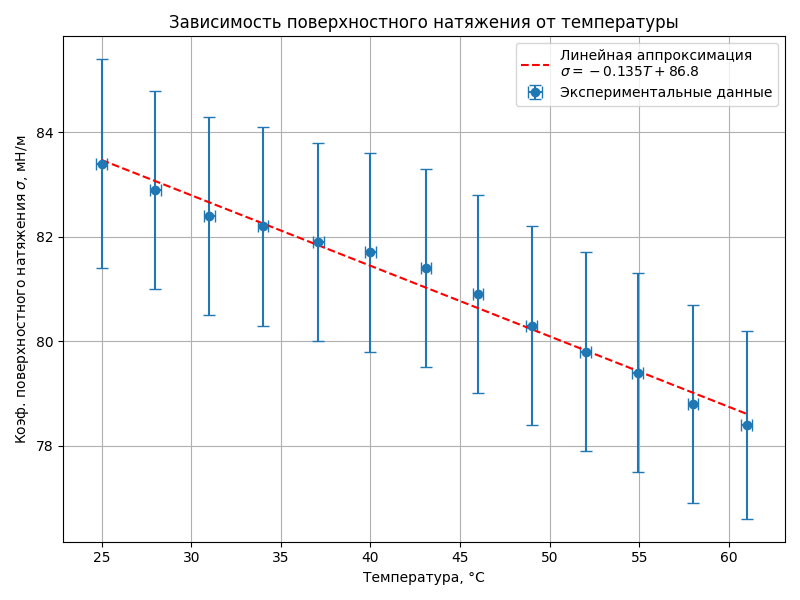
\includegraphics[scale = 0.75]{graph.png}
    \caption{Зависимость $\sigma$ от $T$}
    \label{fig:graph}
  \end{figure}

  \[ 
    \frac{d\sigma}{dT} = - 0.135 \cdot 10^{-3} \, \frac{\text{Н}}{\text{м}\cdot^{\circ}C}
  \]
  
  Оценим погрешность метода наименьших квадратов ($\varepsilon_\text{мнк} = 0.037$) и погрешность прямых измерений.

  \[ 
    \varepsilon_\text{изм} = \sqrt{\varepsilon_\sigma^2 + \varepsilon_T^2} = \sqrt{0.024^2 + 0.003^2} = 0.024
  \]
  \[
    \varepsilon(\frac{d\sigma}{dT}) = 0.037 + 0.024 = 0.061 
  \]
  \[
    d(\frac{d\sigma}{dT}) = 0.061 \cdot (-0.135 \cdot 10^{-3}) = 0.008 \cdot 10^{-3} \, \frac{\text{Н}}{\text{м}\cdot^{\circ}C}
  \]
  Итак,
  \[
    \frac{d\sigma}{dT} = - (1.35 \pm 0.08) \cdot 10^{-4} \, \frac{\text{Н}}{\text{м}\cdot^{\circ}C}
  \]
  
  \item На том же графике изобразим зависимость от температуры теплоты образования единицы площади поверхности $q$ и поверхностной энергии единицы площади поверхности $U/\Pi$.
  
  \[
    q = -T \cdot \frac{d\sigma}{dT}, \qquad \frac{U}{F} = \sigma - T \cdot \frac{d\sigma}{dT}
  \]

  Значения, по которым построен график, приведены в таблице (\ref{tab:last}). Погрешности рассчитываются тривиально: $\varepsilon_q = \sqrt{\varepsilon_T^2 + \varepsilon(\frac{d\sigma}{dT})^2}$ и $d(\frac{U}{F}) = d\sigma + dq$.

  \begin{table}[h!]
    \centering
    \begin{tabular}{|c|c|c|c|}
    \hline
    $T, ^\circ C$ & $\sigma, \frac{\text{мН}}{\text{м}}$ & $q, \frac{\text{мН}}{\text{м}}$ & $U/F, \frac{\text{мН}}{\text{м}}$ \\
    \hline
    25.0 & 83.4 & 3.38 & 86.78 \\
    28.0 & 82.9 & 3.78 & 86.68 \\
    31.0 & 82.4 & 4.19 & 86.59 \\
    34.0 & 82.2 & 4.59 & 86.79 \\
    37.1 & 81.9 & 5.01 & 86.91 \\
    40.0 & 81.7 & 5.40 & 87.10 \\
    43.1 & 81.4 & 5.82 & 87.22 \\
    46.0 & 80.9 & 6.21 & 87.11 \\
    49.0 & 80.3 & 6.62 & 86.92 \\
    52.0 & 79.8 & 7.02 & 86.82 \\
    54.9 & 79.4 & 7.41 & 86.81 \\
    58.0 & 78.8 & 7.83 & 86.63 \\
    61.0 & 78.4 & 8.24 & 86.64 \\
    \hline
    \end{tabular}
    \caption{Таблица значений температуры и соответствующих величин}
    \end{table}

  Сам график изображен на рисунке (\ref{fig:last_graph}).

  \begin{figure}[h!]
    \centering
    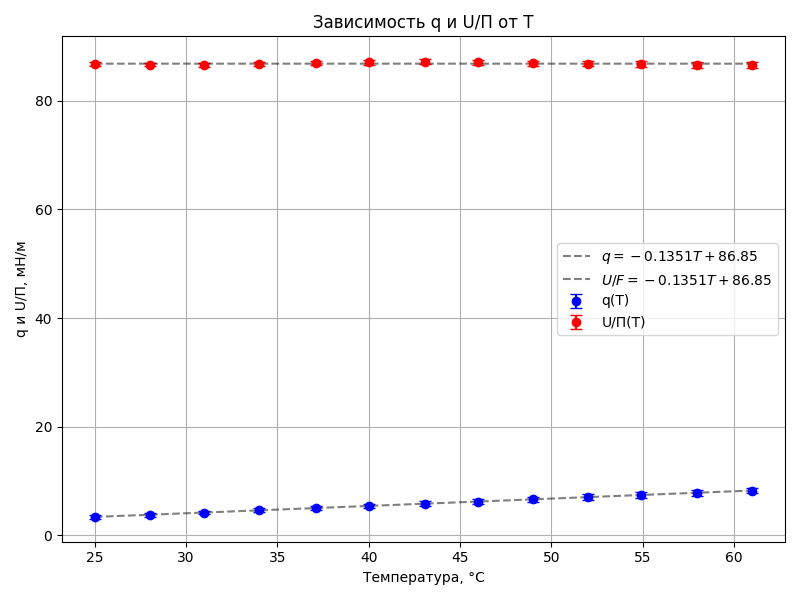
\includegraphics[scale = 0.75]{graph_new.png}
    \caption{Зависимость $q$ и $U$/П от $T$}
    \label{fig:last_graph}
  \end{figure}

  \item Проверим закон Кирхгофа. Будем считать теплоемкость воды постоянной.
  
  \[
    L(T) = L(T_0) + (C_{p \text{(п)}} - C_{p \text{(ж)}}) (T - T_0),
  \]
  где $L(T_0) = 44 \text{кДж}/\text{моль}$, \\
  $\Delta C = C_{p \text{(п)}} - C_{p \text{(ж)}} = -42 \text{Дж}/\text{моль} \cdot K$

  Зная, что $\sigma \sim L$,
  \[
    \sigma = \sigma_0 + k (T - T_0), \qquad k = \frac{d \sigma}{dT}
  \]
  \[ 
    \frac{\left| \frac{d \sigma}{dT} \right|}{\sigma_0} = \frac{\left| C_{p \text{(п)}} - C_{p \text{(ж)}} \right|}{L_0} \sim \frac{\frac{dl}{dT}}{l_0}
  \]

  Построим график $h(T)$ на рисунке (\ref{fig:kirch}). С помощью метода наименьших квадратов определим его угловой коэффициент $k'$. Учтем погрешность метода и погрешность измерений.

  \begin{figure}[h!]
    \centering
    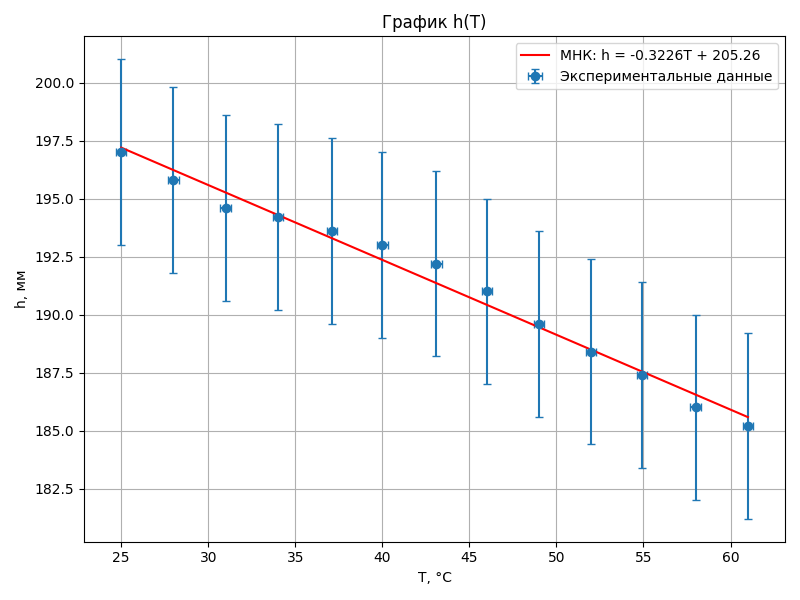
\includegraphics[scale = 0.75]{kirch.png}
    \caption{Зависимость высоты спиртового столбца от температуры}
    \label{fig:kirch}
  \end{figure}
  
\end{enumerate}

\[
  k' = -(0.32 \pm 0.02) \cdot 10^{-3} \, \frac{\text{м}}{K} = -(3.2 \pm 0.2) \cdot 10^{-4} \, \frac{\text{м}}{K} 
\]

Тогда,
\[
  k = \frac{\Delta l}{\Delta T} \frac{\sigma_c}{l_0} = -(1.9 \pm 0.1) \cdot 10^{-4} \frac{\text{H}}{\text{м}\cdot K}, \qquad \varepsilon_k = 0.06
\]

Проверим, выполняется ли соотношение, связанное с законом Кирхгофа:

\[
  \frac{k}{\sigma_0} \approx \frac{|C_{p \text{(п)}} - C_{p \text{(ж)}}|}{L_0}
\]

Подставляя числовые значения:

\[
  \frac{(1.9 \pm 0.1) \times 10^{-4}}{72.0 \cdot 10^{-3}} \approx \frac{42}{44 \times 10^3}, \qquad 2.6 \cdot 10^{-3} \approx 1.0 \cdot 10^{-3}
\]

Оценка дает совпадение в порядке, но значения отличаются примерно в три раза. Выполнение закона Кирхгофа с достаточной точностью подтвердить не удается.

\section*{Вывод}

Все цели работы достигнуты. 

В работе была исследована температурная зависимость коэффициента поверхностного натяжения дистиллированной воды.

Была определена полная поверхностная энергия $U/\Pi$ и теплота $q$, необходимая для изотермического образования единицы поверхности жидкости. 

Проверены законы Лапласа, Паскаля, Кирхгофа.

\end{document}
